\documentclass[a4paper]{article}

\usepackage[utf8]{inputenc}
\usepackage{erk}
\usepackage{times}
\usepackage{graphicx}
\usepackage[top=22.5mm, bottom=22.5mm, left=22.5mm, right=22.5mm]{geometry}

\usepackage[slovene,english]{babel}
\usepackage{hyperref}
\usepackage{url}

\let\oldfootnotesize\footnotesize
\renewcommand*{\footnotesize}{\oldfootnotesize\scriptsize}

\begin{document}
\title{Navodila in osnutek prispevka za končno poročilo pri predmetu Računalniška grafika}

\author{Ciril Bohak$^{1}$, Iztok Lebar Bajec$^{2}$} % use ^1, ^2 for author(s) from different institutions

\affiliation{	$^{1}$Univerza v Ljubljani, Fakulteta za računalništvo in informatiko \\ 
				$^{2}$Univerza v Ljubljani, Fakulteta za računalništvo in informatiko }

\email{E-pošta: ciril.bohak@fri.uni-lj.si}

\maketitle

\selectlanguage{slovene}

\begin{abstract}{Abstract}
Na tem mestu v največ 200 besedah podajte predstavitev svoje igre. Na kratko predstavite idejo, žanr in {upo\-ra\-blje\-ne} tehnologije.
\end{abstract}

% -- Zgolj navodila - to v končni verziji dokumenta odstranite.
\section*{Navodila}
Ta dokument naj vam služi kot osnova za pisanje poročila o seminarju pri predmetu. Končno poročilo ne sme vsebovati več kot 4 strani besedila (skupaj s slikami lahko več), ne sme pa biti krajše od dveh strani vključno s slikami. Slike vključite v dokument kot kaže primer s sliko \ref{fig:slika} in se nanje tudi sklicujte. Prav tako v besedilu predstavite vsebino slik.

\begin{figure}[!htb]
    \begin{center}
        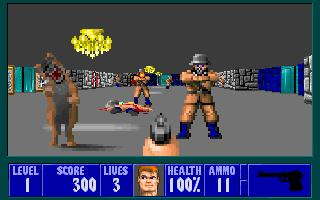
\includegraphics[width=\columnwidth]{wolfenstein.jpg}
        \caption{Kratek opis slike.} \label{fig:slika}
    \end{center}
\end{figure}

Pri pisanju poročila vključujte tudi reference na vire s katerimi ste si pomagali pri izdelavi seminarja. To so lahko pisni viri v obliki knjig \cite{Foley1994}, člankov \cite{Meng2015} ali drugih virov, ki jih dodajte med reference, spletne vire pa navajajte v nogi\footnote{\url{https://en.wikipedia.org/wiki/Computer_graphics}}.

Pri izdelavi igre se omejite na izdelavo enega samega nivoja igre, ki pa ga dodelajte in izpilite kolikor vam do\-pu\-šča predviden čas.

% do sem gre ven



\section{Pregled igre}
V tem poglavju predstavite igro. Za kakšen žanr igre gre. Kakšna je zahtevnost igre. Komu je igra namenjena. V kakšnem okolju se igra odvija. Kakšna je zgodba v igri. Na kratko predstavite tudi sam scenarij igre.

\subsection{Opis sveta}
Na tem mestu podajte grob opis sveta v igri, ki ga podrobenje definirate v sledečih podpoglavjih. Prav tako definirajte v kakšnem stilu bo izdelan svet (npr. realističen, stiliziran, risankast, ipd.). Opredelite tudi ali se bodo osebki v svetu pomikali v eni, dveh ali treh dimenzijah.

\subsubsection{Pregled}
Podpoglavje naj vsebuje podrobnejšo predstavitev sveta, s katerim interaktira uporabnik.

\subsubsection{Ozadje}
Opišite kako je predstavljeno ozadje sveta v igri - predeli s katerimi uporabnik ne interaktira a še vedno predstavljajo del sveta v igri (npr. nebo v ozadju, oddaljeni predmeti ipd.)

\subsubsection{Ključne lokacije}
Izpostavite ključne lokacije v svetu, ki igrajo pomembno vlogo za uporabnika. Navedite zakaj so pomembne, na kakšne način bodo predstavljene (npr. domači tabor, nasprotnikov tabor, nahajališča dobrin  ipd.).

\subsubsection{Velikost}
Dobro opredelite velikost sveta in nivo na katerem bo s svetom interaktiral uporabnik. Kakšen pogled v svet bo primarno zajet v igri (npr. območje mize, sobe, mesta, pokrajine, kontineta, planeta, osončja, ozvezdja, galaksije ipd.)

\subsubsection{Objekti}
Predstavite poglavitne objekte, ki bodo zajeti v igri. Kje ste jih oz. jih boste pridobili. Ali ste jih oz. jih boste izdelali sami ipd.

\subsubsection{Čas}
Opredelite hitrost časa v vaši igri. Kako hitro bodo minevala določena obdobja (npr. 1 dan v igri je 5 minut igralnega časa ali 1 minuta v igri predstavlja 1 uro igralnega časa).

\subsection{Igralni pogon in uporabljene tehnologije}
V poglavju podrobno predstavite katere tehnologije ste uporabili pri izdelavi vašega seminarja. V kolikor ste uporabili kakšno dodatno ogrodje oz. orodje ga na tem mestu predstavite in pojasnite čemu.

\subsection{Pogled}
Definirajte kakšen bo pogled v vašo igro. Kakšno kamero boste uporabili, kaj vse bo uporabnik videl, kako boste poudarjali posamezne stvari ipd.

\section{Osebek}
V tem poglavju podrobno predstavite osebek oz. osebke v igri. Povejte nad katerimi osebki bo imel nadzor uporabnik in nad katerimi ne. Kako se z osebkom oz. osebki upravlja, Kakšne so akcije osebka ipd.

\section{Uporabniški vmesnik}
Poglavje naj podrobno predstavi uporabniški vmesnik. Od izgleda pa do same implementacije in interakcije. Utemeljite zakaj ste uporabili takšen vmesnik kot ste ga.

\section{Glasba in zvok}
V kolikor v igri uporabite glasbo in zvok predstavite ka\-kšna glasba je v vaši igri in zakaj. Ali se glasba prilagaja posameznim situacijam? Kako je z zvočnimi efekti? Kje ste jih pridobili? Kje uporabili?

\section{Gameplay}
Nenazadnje predstavite tudi sam gameplay - potek igranja vaše igre. Kako se igra prične in na kakšne načine jo lahko zaključimo? Kakšne akcije so uporabniku na voljo med samo igro in na kaj vplicajo?


\section{Zaključki in možne nadgradnje}
V poglavju povzemite česa ste se pri izdelavi igre naučili. Ali ste pri predmetu pridobili dovolj znanja oz. kje je bilo pomanjkanje? Povzemite tudi do kakšnih razlik je prišlo med predvidenim scenarijem in končno izvedbo igre.


\small
\bibliographystyle{plain}
\bibliography{references}

\end{document}
